\documentclass[12pt]{beamer}
\author{Yan Wang}
\title{Paper Reading Seminar}
\subtitle{}
\usetheme{Malmoe}
\setbeamertemplate{navigation symbols}{}
\newcommand*\oldmacro{}%
\let\oldmacro\insertshorttitle%
\renewcommand*\insertshorttitle{%
\oldmacro\hfill%
\insertframenumber\,/\,\inserttotalframenumber}

\begin{document}

\begin{frame}[plain]
    \titlepage
\end{frame}

\begin{frame}{Image Matching via Saliency Region Correspondences}
    \begin{itemize}
        \item Intuition
        \begin{itemize}
            \item Segmentation is not perfect. Weak connections $\Rightarrow$ graph-based segmentation (NCut)
            \item Matching is not perfect. Weak connections $\Rightarrow$ spatial consistency check
            \item Combine the two tasks together $\Rightarrow$ use a single graph to get a joint optimal
            \item Encoding context in the matching process $\Rightarrow$ no need for spatial consistency check
        \end{itemize}
        \item Outline
        \begin{itemize}
            \item Formulation
            \item Optimization
            \item Features
        \end{itemize}
    \end{itemize}
\end{frame}

\begin{frame}{Formulation}
    \begin{itemize}
        \item Graph formulation
        \begin{itemize}
            \item Vertex: pixel
            \item Layer: two-layer, one for each image
            \item Intra-layer edges: how strongly the pixels are similar (connected) in this image
            \item Inter-layer edges: how strongly the pixels are similar (connected) across images
            \\ \medskip { 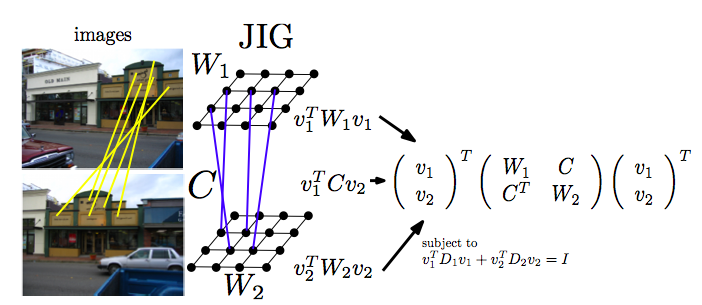
\includegraphics[width=0.7\textwidth]{graph-framework.png} \\ } 
        \end{itemize}
    \end{itemize}
\end{frame}

\begin{frame}{Formulation}
    \begin{itemize}
        \item Intra-layer optimization goal
        \[\max_v \frac{v_1^TW_1v_1 + v_2^TW_2v_2}{v^TDv}\]
        \begin{itemize}
            \item Binary segmentation problem (extend to multi-class with 1-vs-all binary mask)
            \item Each segment should be internally consistent $\Rightarrow v_1^TW_1v_1$. Only if $v_{1j}, v_{1k}$ both positive, will $W_{1(i,j)}$ be counted
            \item $v_{i} = \{0, 1\}^{n_i}, \sum_j v_{ij} = 1$, indicator vector for image $i$, pixel $j$, and cluster $k$, $v = [v_1^T, v_2^T]^T$
            \item Normalize on the size: $\sum_j v_{1j}^TW_1$ = ${\bf 1}^TW_1 = D_1$
        \end{itemize}
    \end{itemize}
\end{frame}

\begin{frame}{Formumation}
    \begin{itemize}
        \item Inter-layer optimization goal
        \[\max_v \frac{v_1^TCv_2}{v^TDv}\]
        \begin{itemize}
            \item ``Co-saliency'' regions (where $v_{ij} = v_{ik}$) should be similar
            \item Also normalize on size
            \item Use ``context'' to refine segmentation as well as matching
        \end{itemize}
    \end{itemize}
\end{frame}

\begin{frame}{Formulation and optimization}
    \begin{itemize}
        \item Final optimization goal
        \begin{itemize}
            \[F(v^{(c)}, C) = \text{IntraIS}(v^{(c)}, C) + \text{InterIS}(v^{(c)}, C)\]
            \item $v^{(c)}$: binary segmentation result for the $c$th segment.
        \end{itemize}
        \item Relaxation for optimizaiton
        \begin{itemize}
            \item $v$ to real vector
            \item Joint ``soft'' segmentation result $V$ (set of eigenvectors) lies in the subspace spanned by the individual ``soft'' segmentation results $S_1$ and $S_2$.
            \item Relax the synchronization with orthogonal constraints.
            \item EM iterative optimization, with no explicit proof of convergence (in some speicial cases, EM algorithms can arrive in stationary points)
        \end{itemize}
    \end{itemize}
\end{frame}

\begin{frame}{Features}
    \begin{itemize}
        \item MSER detector + SIFT descriptor
        \item Intra-image $W$
        \begin{itemize}
            \item $x, y$ are considered in the same segment $\Leftrightarrow$ no edges with large magnitude spatially separate them
            \item Edge detection with large magnitude $\Rightarrow$ get $W$
        \end{itemize}
        \item Inter-image $C$
        \begin{itemize}
            \item 1. Feature detection: also consider the ellipse (orientation/scale) from the detector
            \item 2. Feature matching
            \item 2.0 Simplest pixel-wise matching: Gaussian kernel + descriptor + ellipse matrix
            \[m_{x, y}(p, q) = e^{-\lVert d_p - d_q \rVert^2/\sigma_i^2}e^{-\lVert H_p(x)-H_q(y)\rVert^2/\sigma_p^2}\]
        \end{itemize}
    \end{itemize}
\end{frame}

\begin{frame}{Features}
    \begin{itemize}
        \item Inter-image $C$
        \begin{itemize}
            \item 2.1 Adopt patch-wise feature matching score as pixel-wise score for $C$
            \[M_{x, y} = \max\{m_{x, y}(p, q) \ | \ p\in P, q \in Q, x \in R_p, y \in R_q\}\]
            One point can be involved in multiple MSER interest regions. For every point pair $x, y$, check all the MSER pairs (with different $H$ settings), and pick up the highest matching score
            \item 2.2 Compute patch-wise similarity matrix $M$, and then normalize to $C$
            \[D^{-1/2}_1CD^{-1/2}_2 = P \circ M\]
        \end{itemize}
    \end{itemize}
\end{frame}

\end{document}
